% mainfile: ../RobertoDiRemigioPhDThesis.tex
%************************************************
\chapter{Summary of the publications}\label{ch:publications-summary}

\epigraph{\textonehalf\,\,research \kern 20pt and \textonehalf \kern 20pt \textgreek{Tέχνη}

          \textonehalf\,\,observation, \kern 22pt \textonehalf \kern 20pt \textgreek{Tέχνη}

          \textonehalf\,\,training, \kern 39pt \textonehalf \kern 20pt \textgreek{Tέχνη}
          }{
  --- \textsc{Ezra Pound}, \textit{Canto LXXXV}}

This final Chapter provides a brief overview of the motivations, results and
conclusions of the papers this thesis is based on.
All publications included in this thesis have involved some programming effort.
I will also describe the principles we have striven to follow in developing our
\acs{PCM} software library and its management philosophy.
I will also give some details on the interfaces we have developed to different
quantum chemistry codes.
Finally, for each paper, I will give a description of my contributions to the
work leading to its publication.
\todo[inline]{Write something along these lines: "My coauthors have all read and approved."}

\pagebreak

\refstepcounter{dummy}
\addcontentsline{toc}{section}{Software}
\section*{Software}

\todo[inline]{Have a closer look at this. I think it needs to be updated for the discussion
on open-source software that went down on JPC Lett. some time ago.
Also, acronyms should be properly set up.}

A shorter version of this discussion has been accepted for publication in the
proceedings of the \emph{Producing High Performance and Sustainable Software
for Molecular Simulation} workshop held at the 2015 Supercomputing Conference.

We have created an open-source, standalone library to provide \acs{PCM} functionality across
altogether different quantum chemical program packages.
The library serves as our development platform for the \acs{PCM}.
Moreover, the interfaces developed to different quantum chemistry codes allow the exploration
of new methodologies, significantly cutting down development times.

\begin{figure}[!htb]
\centering
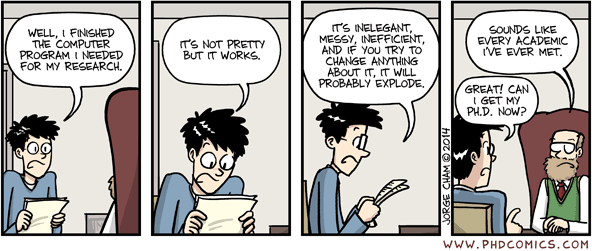
\includegraphics[width=.8\textwidth]{notpretty.png}
\end{figure}

The codes used in the papers are all interfaced to the \pcmsolver library,
of which I am the main developer and maintainer.

\begin{figure}[!htb]
\centering
\scalebox{0.8}{\tikzstyle{decision}=[diamond, fill=brewerRed!20, text width=5.5em, text badly centered, inner sep=0pt]
\tikzstyle{pcmsolver}=[rectangle, minimum size=10mm, rounded corners=3mm, very thick, fill=brewerBlue!20, text width=15em, text centered]
\tikzstyle{qmprog}=[rectangle, minimum size=10mm, rounded corners=3mm, text centered, very thick, fill=Green!20, text width=15em]

\begin{tikzpicture}[]
%skip up/.style={to path={-- ++(0,#1) -| (\tikztotarget)}},
%skip right/.style={to path={-- ++(#1,0) -| (\tikztotarget)}}]
\node (MEP) [qmprog] { Molecular electrostatic potential: \\ $\esp(\vect{s})$};
\node (CHG) [pcmsolver, below=of MEP] { Apparent surface charge:\\ 
$\bi{R}_\diel\bi{S}\sigma(\vect{s}) = - \bi{R}_\infty\esp(\vect{s})$ };
\node (energy) [pcmsolver, below=of CHG] { Polarization energy:\\ 
$U_\mathrm{PCM} = \frac{1}{2}\scalprod{\sigma(\vect{s})}{\esp(\vect{s})}$};
\node (fock) [qmprog, below=of energy, distance=30mm] { Fock matrix:\\
$f_{\kappa\lambda} = f^\mathrm{vac}_{\kappa\lambda} + \scalprod{\sigma(\vect{s})}{\esp_{\kappa\lambda}(\vect{s})}$ };
%\node (iter) [qmprog, below=of fock, distance=150mm] { Iterate SCF };
\node (conv) [decision, below=of fock] { SCF converged?};
\node (end) [qmprog, below=of conv] { Finalize SCF};
\path (MEP) edge[->] (CHG)
      %(nucchg) edge[->] (elepot)
      %(elepot) edge[->] (elechg)
      (CHG) edge[->] (energy)
      (energy) edge[->] (fock)
      (fock)   edge[->] (conv)
 %     (iter)   edge[->] (conv)
      (conv)   edge[->] node[anchor=east]{yes} (end);
\draw [->] (conv.east) -- ++(1,0) node[anchor=south] {no} --++(1,0) |- (MEP.east);
\draw [<-] (MEP.west) -- ++ (-1,0) node[anchor=south]
      {\textcolor{brewerBlue}{Cavity}} node [anchor=north] {\textcolor{Green}{\!\!\!\!Geometry}, \textcolor{Green}{$\mat{D}$}} -- ++(-1,0);
\draw [<-] (CHG.west) -- ++ (-1,0) node[anchor=south] {\textcolor{brewerBlue}{BE solver}} -- ++(-1,0);
\end{tikzpicture}
}
\caption[Modular approach to programming a \acs{PCM} functionality into an existing \acs{SCF} code.]{
  Schematic view of the implemented SCF algorithm. Computations/data in
  \textcolor{Blue}{blue} are on the \pcmsolver side, in
  \textcolor{Green}{green} on the \DIRAC side.
  }
\label{fig:algorithm}
\end{figure}

The growing complexity of quantum chemical program packages requires that an
appropriate strategy be devised to implement new features.
Scalability is of paramount importance, but it has become clear that
maintainability and extensibility of the code play an equally important role in
managing this growing complexity.~\autocite{Hatton1994-us, Hatton1997-ml,
Hatton1997-bb, Ioannidis2005-aj, Merali2010-uy, Prinz2011-kz, Wilson2014-vh}

The use of a \emph{modular programming paradigm} has been recognized as
beneficial in many other scientific computing contexts. New features are
isolated into libraries that can be accessed by host programs through a
well-defined \ac{API}.
Computational tasks are thus implemented into separate, independent and
interchangeable modules. These are \emph{developed} and \emph{tested}
independently of the particular host program in which they will be
used.~\cite{Dijkstra1968-zp, Parnas1972-im}
A well-defined \ac{API} clearly delimits the boundaries of the functionality
offered, thus forcing a programming style and standardisation of the
functionality, eventually.~\autocite{Reddy2011-sd}

When coupled with \emph{open-source} licensing, modularity is a proper
step towards ensuring reproducibility of results from scientific
simulation software \cite{Gezelter2015-gz, Krylov2015-fs, Jacob2016-oq}.
Open-source development can fully leverage the benefits
of widespread, cloud-based, free, code development services, such as
hosted \acp{DVCS}, \ac{CI}, code
coverage, static and dynamic code analyses, nightly regression testing,
public issue tracking, code review and so forth:
adoption of a modern code development workflow is easily within reach.

It is, of course, true that the above mentioned services are not
exclusive prerogatives of open-source projects.
However, an open review process of scientific software can often help
to establish
reproducibility, extensibility and sustainability of the software
ecosystem.
Open-source software, modular development of new functionalities
and full-fledged exploitation of \acsp{DVCS} ensure a much larger scientific
impact. Third-parties can easily contribute to
the project: by improving the documentation, by reporting bugs or
by actively extending the codebase with new functionality.

The description of chemical phenomena in complex environments, such as
solutions or proteins, is as challenging as it is important
for an accurate prediction of a wide range of properties.~\autocite{Reichardt2010-le}
  Quantum chemistry is nowadays a valuable
tool: its simulations can provide significant insight into complex
chemical phenomena.~\autocite{Nobel1998, Nobel2013}.
The major challenge lies in providing a faithful, realistic, yet cost-effective
description of the environment of the molecule:
a molecule in solution can be represented by a quantum mechanical model
comprising a great number of atoms, thousands or more. Such a simulation would,
however, be impossible to carry out with the current state-of-the-art
computational resources.
Models must be devised to overcome the dimensionality ``disease'' and
the idea of introducing different approximation levels for different
parts of the system under study is particularly appealing, as it helps
our chemical understanding. This is the idea at the basis of
\emph{multiscale} models.

\begin{figure}[!htb]
  \centering
  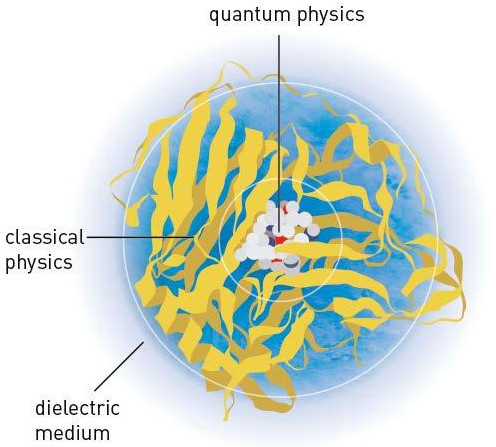
\includegraphics[width=.45\textwidth]{multiscale.jpg}
\end{figure}

\emph{Continuum} (or \emph{implicit}) models, deal explicitly
only with the degrees of freedom associated with the solute, while
replacing the solvent with a structureless continuum characterized by
its bulk properties \cite{Onsager1936-wf}. Among these models, the \acl{PCM} (\acs{PCM})
is the most widespread and successful \cite{Tomasi2005-vm, Mennucci2008-xl}.

The \acs{PCM} is also an ideal candidate for the creation of a solvation \acs{API}.
Its input from and output to \emph{any} quantum chemistry code is
limited and well-defined.
This provides a natural \acs{API} design: the \acs{API} functions can be compared
\emph{vis-à-vis} with the working equations derived for the different
quantum chemical methods.

We will elucidate the design principles adopted in the development of our
\pcmsolver library: an \emph{open-source} \acs{API} for the inclusion of the
PCM in \emph{any} quantum chemistry code \cite{PCMSolver}.  Use of our
\acs{API} \emph{significantly} limits coding effort on the side of the host:
continuum solvation at the \acs{SCF}
level of theory can be implemented in the host program almost out-of-the-box.  The module is
agnostic of the host code internals and is tested separately from it.

We will emphasize the role of the open-source licensing model and the
importance of the modern workflows adopted in our project.  The adoption
of \git as \acs{DVCS}, \cmake for cross-platform builds and automatic
documentation deployment on \readthedocs simplify extensibility of the
module and promote third-party contributions to the code base, while
continuous integration and nightly testing offer an invaluable level of
confidence in the code.

\begin{figure}[!htb]
  \centering
  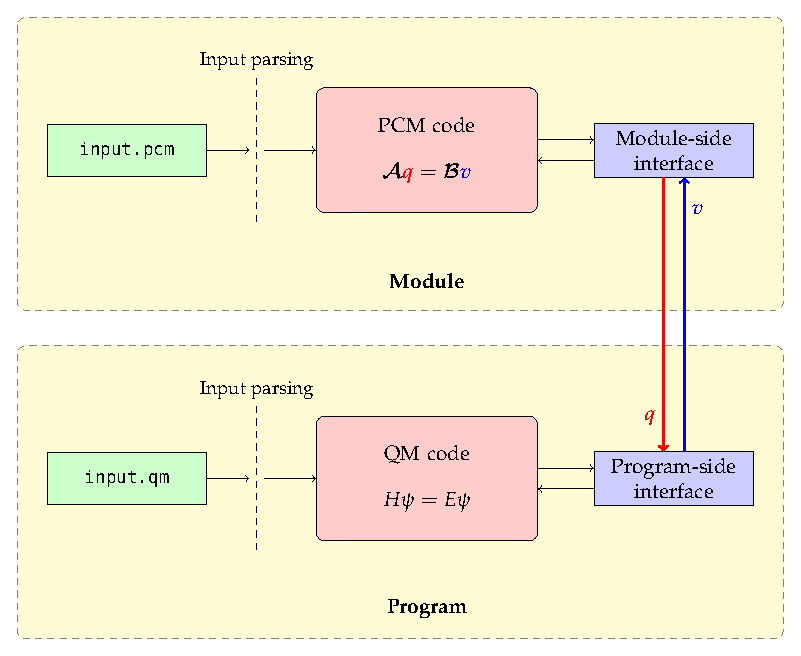
\includegraphics[width=.5\textwidth]{pcmsolver-scheme}
\end{figure}

\pcmsolver currently offers the basic PCM functionality already
available in many widespread software packages, such as traditional
collocation solvers for isotropic media.~\autocite{Tomasi2005-vm}
Some unique functionalities are the wavelet Galerkin solvers on smooth
molecular surfaces~\autocite{Weijo2010-hy, Bugeanu2015-tp}, the Green’s
functions for spherical diffuse interfaces~\autocite{DiRemigio2016-nn} and
the delayed solvers for real-time \acl{TDSCF}
simulations.~\autocite{Corni2015-pe}

Careful usage of the C++ object-oriented paradigm is the key to this
wide spectrum of functionalities. The library is in itself made of
modules, communicating by means of composition at the outermost
level of the design.
This allows us to mix languages internally: we currently have Fortran
and C modules alongside the main C++ structure.
Library internal classes balance the dynamic polymorphism offered by
inheritance and the static polymorphism offered by template programming.
~\autocite{Alexandrescu2001-bp, Sutter2004-nt, Langr2012-js}
Preeminent use of composition over inheritance keeps the coupling
between different modules as low as possible.~\autocite{Gamma1995-fd}

References for the various codes we have created interfaces to.
\psicode~\autocite{Turney2012-de}
\DIRAC~\autocite{DIRAC15}
\DALTON~\autocite{DALTON16, Aidas2013-rp}
\LSDALTON~\autocite{LSDALTON16, Aidas2013-rp}
\ReSpect~\autocite{ReSpect-3.5.0, OtherStuff}
KOALA~\autocite{Hofener2014-ex, Hofener2016-qz}

\refstepcounter{dummy}
\addcontentsline{toc}{section}{Continuum solvation in the relativistic regime}
\section*{Paper I. Continuum solvation in the relativistic regime}

Systems containing heavy elements are notoriously challenging for quantum chemistry.
In addition to their significantly large sizes, one has to properly include the
effect of special relativity in the quantum chemical description in order to
achieve at least qualitative agreement with experiment.
Additional complications arise if one needs to also include environment effects.
Continuum models arguably represent a cost-effective strategy to achieve a first
approximation of these effects.
In this paper, we presented the first derivation and implementation of the \acs{PCM}
coupled to a \acs{SCF} description of the solute in the fully relativistic, four-component
regime.
Our preliminary calculations on the group 16 dihydrides \ce{H2X} (\ce{X} =
\ce{O}, \ce{S}, \ce{Se}, \ce{Te}, \ce{Po}) have shown that the method predicts
a noticeable interplay of relativistic and solvent effects when heavier
elements are involved.
The main point of the paper was, however, the adoption of a fully modular
programming strategy. We showed that it is entirely possible to adopt the same
\acs{PCM} code and implementation "checkpoints" across altogether different
problem domains, Fig.~\ref{fig:algorithm}.

As a by-product of the four-component implementation, we were able to obtain and visualize \acs{MEP} maps
from four-component \acs{SCF} wave functions. These add yet another interpretive tool to the toolbox available
in the four-component relativistic regime.
The interface to \DIRAC was later released in the 2014 and later versions,
providing \acs{PCM} capabilities to the software package.

I contributed the theoretical derivation of the quantum/classical polarizable
terms in a four-component \acs{SCF} framework, for energies and linear response
properties. I devised the coupling of the four-component program \DIRAC with
\pcmsolver by providing the implementation and testing of:
\begin{enumerate*}[label={\alph*)},font={\color{PMS1797}}]
  \item \acs{MEP} integrals for four-component wave functions,
  \item the additional Fock matrix contributions and
  \item the additional terms in the response equations.
\end{enumerate*}
I performed all the calculations and large part of the data analysis
for the results reported in the paper.
Finally, I wrote the first draft of the paper and coordinated editing of
all subsequent versions.

\refstepcounter{dummy}
\addcontentsline{toc}{section}{The wavelet Galerkin boundary element method for PCM}
\section*{Paper II. The wavelet Galerkin boundary element method for PCM}

Continuum solvation models are inherently parametrized. Apart from solvent permittivities,
the atomic radii and molecular surface definition play a crucial role
in determining the performance of the models.
However, the numerical accuracy of the \acs{BEM} procedure used to numerically solve the
underlying \acs{BIE} is a not-so-often studied aspect of these models.
Traditionally, collocation methods have been used, but these require parametrization of some of the necessary surface integrals.
Galerkin methods do not suffer from such a limitation and additionally preserve symmetry of the underlying
boundary integral operators.
The use of biorthogonal wavelet bases as finite elements achieves sparsity in
the \acs{BEM} procedure, due to their intrinsically hierarchical structure and
the existence of \emph{a priori} and \emph{a posteriori} matrix compression
estimates.
Thus, wavelet Galerkin \acs{BEM} represents a valid alternative to traditional
collocation methods, both to achieve a better computational scaling and to
provide accurate, benchmark results.\autocite{Harbrecht2004-uo,
Harbrecht2006-ug, Dahmen2006-pj}

Already~\citeauthor{Weijo2010-hy} had shown that using \ac{PWC} bases can lead
to superior accuracy and convergence in the calculation of quantum mechanical
molecular solvation energies.
In this work we showed that even faster convergence can be achieved when
\ac{PWL} bases are used instead.
Moreover, the same holds for the calculation of static electric properties.
Notably, the traditional collocation solver cannot guarantee the same accuracy,
even for very large finite element bases. This suggests that, in some cases,
\acs{BEM} collocation methodologies might slow down or even prevent the
convergence of the quantum mechanical response equations solvers.

For this paper, I provided template interface and test sets for the cavity
generator\autocite{Harbrecht2009-no, Harbrecht2011-dk} and wavelet Galerkin
\acs{BEM} solver\autocite{Harbrecht2004-uo, Harbrecht2006-ug} with \pcmsolver.
These were used to interface with the new C++ implementation of the wavelet
Galerkin solvers of Monica Bugeanu.
I implemented the interface between the \LSDALTON quantum chemistry software
package and the \pcmsolver software library. The interface allows to run \acs{HF} and
\acs{KS}-\acs{DFT} single-point and linear response calculations.
Together with coauthor Krzysztof Mozgawa, I performed the benchmark quantum
chemical calculations presented in the paper.
Finally, I coordinated the editing of all manuscript drafts.
In particular, I wrote the first draft of Sections 2.1 and 2.3.
The first draft of Sections 3 and 4 was co-written with the first author, Monica Bugeanu.
I performed most of the data analysis and produced tables and graphs.

Finally, the interface to \LSDALTON was later released in the 2016 version,
providing \acs{PCM} capabilities to the software package.

\refstepcounter{dummy}
\addcontentsline{toc}{section}{Non homogeneous environments}
\section*{Paper III: Non homogeneous environments}

Continuum solvation models offer a simple route to the treatment of non
homogeneous environments.
The general integral equation formulation is in fact transparent with respect
to the definition of the Green's function for the space portion exterior to the
cavity.
As outlined in Chapter \ref{ch:CSM}, the boundary integral operators in the
\acs{IEF} equation:
\begin{equation}
  \left[ \bi{S}_\mathrm{e}\left(2\pi + \bi{D}^\dagger_\mathrm{i}\right)
  +
  \left(2\pi - \bi{D}_\mathrm{e}\right)\bi{S}_\mathrm{i}
  \right]\sigma =
  -\left[\left(2\pi-\bi{D}_\mathrm{e}\right)
  -\bi{S}_\mathrm{e}\bi{S}_\mathrm{i}^{-1}
  \left(2\pi-\bi{D}_\mathrm{i}\right)
  \right]\esp,
  \tag{\ref{eq:full-IEF} from Chapter \ref{ch:CSM}}
\end{equation}
can be set up once the Green's functions $\Gi$ and $Ge$ are known.~\autocite{Cances1998-og}
\citeauthor{Frediani2004-er} showed that a numerical representation of the
Green's function is sufficient to obtain the boundary integral operators in the
\acs{PCM} integral equation.
The authors introduced a numerical integration procedure to calculate the
Green's function for an environment characterized by spatially varying, yet
cilindrically symmetric, permittivity functions: a model for planar diffuse interfaces.

In this work, a similar procedure was introduced to tackle diffuse interfaces
in spherical symmetry.
In contrast to previously existing work, our implementation offers a more robust
treatment of thin interfaces, with a rather generic functional form for the
permittivity profile.
We thoroughly analyzed the necessity for the \emph{a posteriori} removal of the
Coulomb singularity from the computed Green's function and its efficient
implementation.
Interface width and curvature influence the transfer of ions and molecules across
spherically symmetric interfaces and peculiar properties may arise.
In this work, we analyzed both effect on the water-vapor and oil-water transfer
of \ce{Li+}, \ce{Br-}, acetone, \emph{para}-nitroaniline and the L0 dye.
Nonelectrostatic interactions were not included in our implementation, although
they have been proved to be crucial for non homogeneous
environments.~\autocite{Mozgawa2014-ad}
Nevertheless our implementation represents a first significant step in the continuum treatment
of such nontrivial environments.

I contributed the theoretical work for this paper, based on earlier drafts from coauthors
Ville Weijo and Hui Cao. In particular, I derived the separation of
the Coulomb singularity in its final form.
Moreover, I contributed the implementation and testing of the Green's function code.
The interface to the \LSDALTON program package, developed within paper II, was
also used for this paper.
I wrote the first draft of the paper and coordinated all subsequent editing stages.

\refstepcounter{dummy}
\addcontentsline{toc}{section}{Relativistic Calculation of EPR and pNMR Parameters in Solution}
\section*{Paper IV: Relativistic Calculation of EPR and pNMR Parameters in Solution}

Paper IV is a step further in our exploration of the interplay between
relativistic and solvent effects initiated with Paper I.
Whereas Paper I presented the essential framework for the coupling of
four-component \acs{SCF} wave functions with a classical polarizable continuum,
in this paper we explored the calculation of first-order magnetic properties:
\ac{EPR} and \ac{pNMR} parameters.~\autocite{Repisky2010-ls, Malkin2011-nm,
Komorovsky2013-xa, Cherry2016-ij}
The two works are thus complementary since they explore two different classes
of properties and present implementations in two algorithmically different
relativistic quantum chemistry codes.
In the relativistic framework, spin-orbit interactions are included from the
outset in the variational optimization of the wave function.
Hence, \acs{EPR} and \acs{pNMR} parameters are formulated as expectation
values, by virtue of the Hellmann--Feynman theorem.~\autocite{Konishi2009-zb,
Helgaker2000-tz}
Moreover, the \ReSpect code can exploit the \emph{Kramers unrestricted} formalism,
allowing for spin polarization and thus granting facile access to the computation
of spin-dependent properties.~\autocite{Dyall2007-tu}
The same modular programming strategy was adopted in crafting an interface between the
relativistic four-component code \ReSpect\autocite{ReSpect-3.5.0} and \pcmsolver.

My contributions to this paper include prototyping the interface between the
\pcmsolver library and the \ReSpect quantum chemistry code.
The interface is maintained in collaboration with coauthor Michal Repisky, who also
refined the implementation to achieve better computational performance.
I tested the interface against one-component and four-component results obtained with
the \LSDALTON and \DIRAC codes, respectively.
I helped coauthors Michal Repisky, Stanislav Komorovsky and Peter Hrobarik
with setting up the \acs{PCM} calculations described in the paper.
Finally, I provided the first draft for Section 2 of the paper and took part in all editing stages.
The interface to \ReSpect will be released in the next public version of the software
package, providing \acs{PCM} and \acs{COSMO} capabilities.

\refstepcounter{dummy}
\addcontentsline{toc}{section}{Open-ended self-consistent field response theory in solution}
\section*{Paper V: Open-ended self-consistent field response theory in solution}

In recent years, the availability of strong lasers has allowed to
design and carry out experiments where the high-order response of
molecular materials can be routinely probed.
The more intense the light source, the more complicated the interpretation of
the measured signal.
Our group has newly developed an open-ended methodology for the computation of
\acs{SCF} response functions~\autocite{Thorvaldsen2008-sg, Ringholm2014-gx} and
their residues.~\autocite{Friese2015-kb}
These developments offer a route towards a synergistic experimental and
theoretical approach to high-order absorption spectroscopies.
Paper V grafts a classical polarizable continuum approach to solvation on top
of the open-ended methodology of \citeauthor{Thorvaldsen2008-sg}.
Still nowadays, continuum models represent a cost-effective methodology for the
approximate inclusion of solvent effects, albeit their known limitations with respect
to specific solute-solvent interactions.

I developed the theoretical framework for the open-ended \acs{SCF} formulation
of molecular response properties when a quantum/classical polarizable continuum
Hamiltonian is used.~\autocite{Thorvaldsen2008-sg, Lipparini2010-be}
I provided its implementation within the \DALTON code, by interfacing the
\pcmsolver library and the open-ended \acs{SCF} response code of
\citeauthor{Ringholm2014-gx}~\autocite{Ringholm2014-gx, Friese2015-kb}
I performed extensive testing of the code by comparing with previously
published implementations of the \acs{PCM}-\acs{SCF} response functions within
\DALTON.~\autocite{Cammi2003-qy, Frediani2005-nc, Ferrighi2010-pm}
Together with coauthors Maarten T.~P.~Beerepoot and Yann Cornaton, I carried out
the multiphoton absorption calculations presented in the paper. I contributed
to data collection and data analysis.
I drafted the initial versions of Sections 2 and 3 of the manuscript and coordinated all
editing stages with coauthor Maarten T. P. Beerepoot.
